\section{Task Planning (Jim)}

The high-level planner in this work serves as the ``brain'' of the whole framework.
It takes an input of the {\it configuration file} and automatically generate and execute an assembly plan to place given modules as specified in the {\it configuration file}.
Fig.~\ref{fig:taskplan} shows the overview structure of the high-level task planner.

\begin{figure}[ht!]%[H]
\centering
{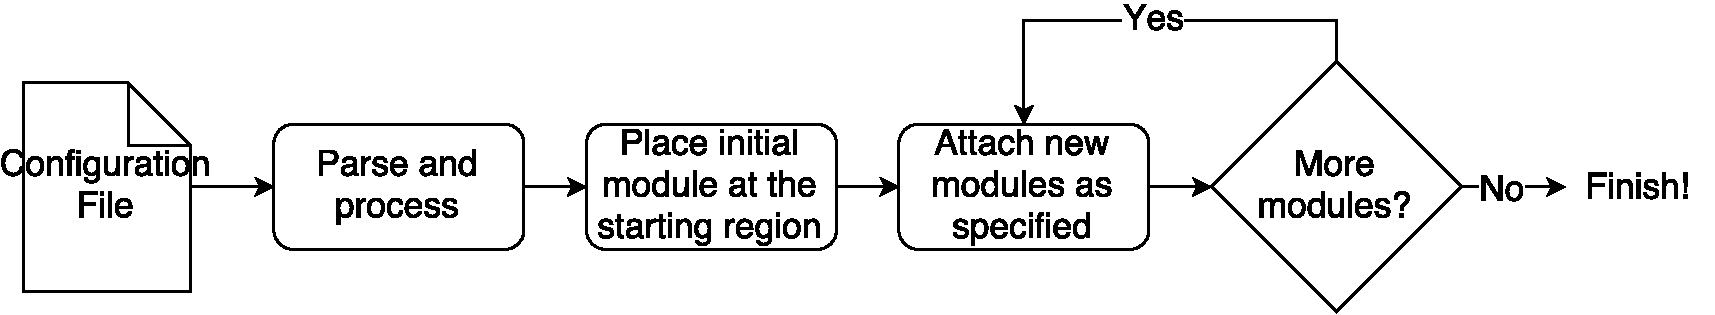
\includegraphics[width=0.95\columnwidth]{pics/highlevelflow.pdf}}
\caption{High-level Task Planning Module}
\label{fig:taskplan}
\end{figure}

\subsection{Parse and process the configuration file}
To specify the desired configuration of the modular robots, a user can use an existing designer VSPARC ({\color{red}cite}) to design the configuration and generate a {\it configuration file} that encodes information of the connectivity among all modules.
Fig.~\ref{fig:configfile} shows an sample {\it configuration file}.

\begin{figure}[ht!]%[H]
\centering
{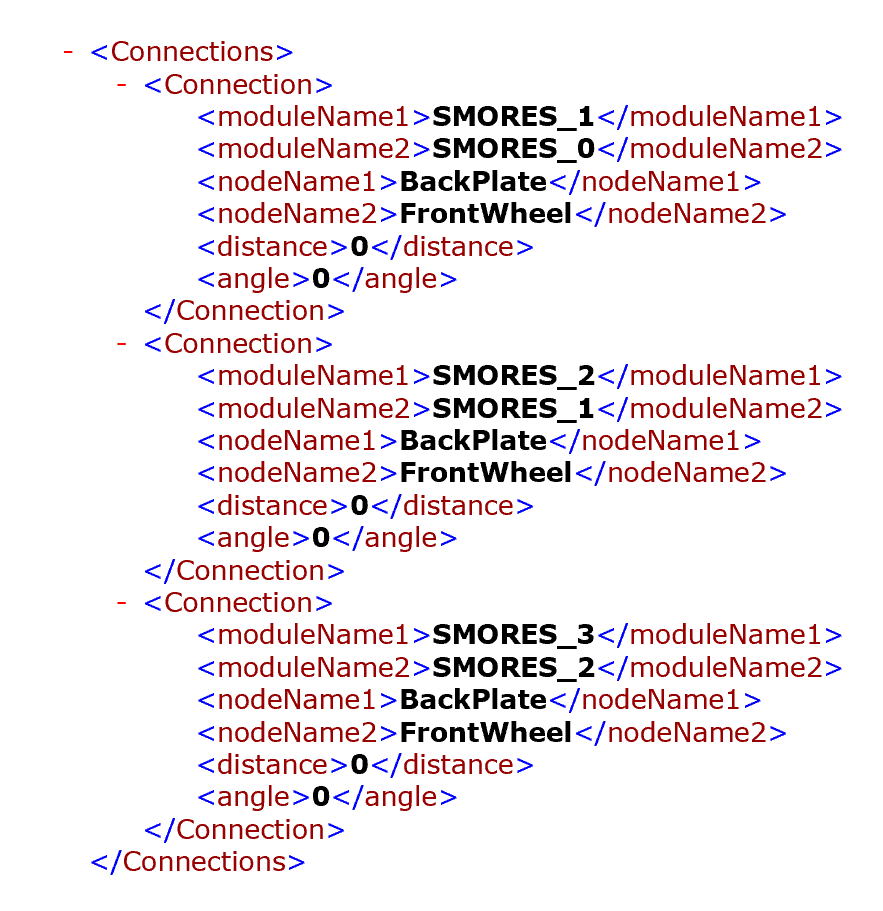
\includegraphics[width=0.95\columnwidth]{pics/configfile.png}}
\caption{A sample configuration file}
\label{fig:configfile}
\end{figure}

The high-level planner can parse the {\it configuration file} and build a graph encodes all connections.

\subsection{Place initial module at the starting region}
To start the assembly, an initial module needs to be selected and placed at the starting region.
\subsubsection{Select initial module}
Consider the scenario shown in Fig.~\ref{fig:loop}. Eight modules are placed at locations in blue.
It is hard to place a new module at the center location in red, as it is  fully surrounded by eight modules. Therefore, we decide to assemble modules in the order such that modules located in the center of the configuration are placed before modules located at edges of the configuration.
To achieve this guarantees, we rank all modules based on the number of connections each module has. The maximum connection a module can has is four.
Therefore, all modules are separated into four ranks. The higher the rank, the more connections a module has. 
When choosing the initial module, we will prefer the module in a higher rank. 
If there are more than one module in a rank, we will prioritize the module with more high rank neighbors.
This selection method is also utilized when choosing the next module to be placed as describe in Section~\ref{sec:nextmodule}.
With this ranking method, we might still encounter difficulty when solving the scenario in Fig.~\ref{fig:loop2}.
When the configuration is a 7-by-7 square made of 49 modules, we do not have difference in preference among modules in red.

\begin{figure}[ht!]%[H]
\centering
{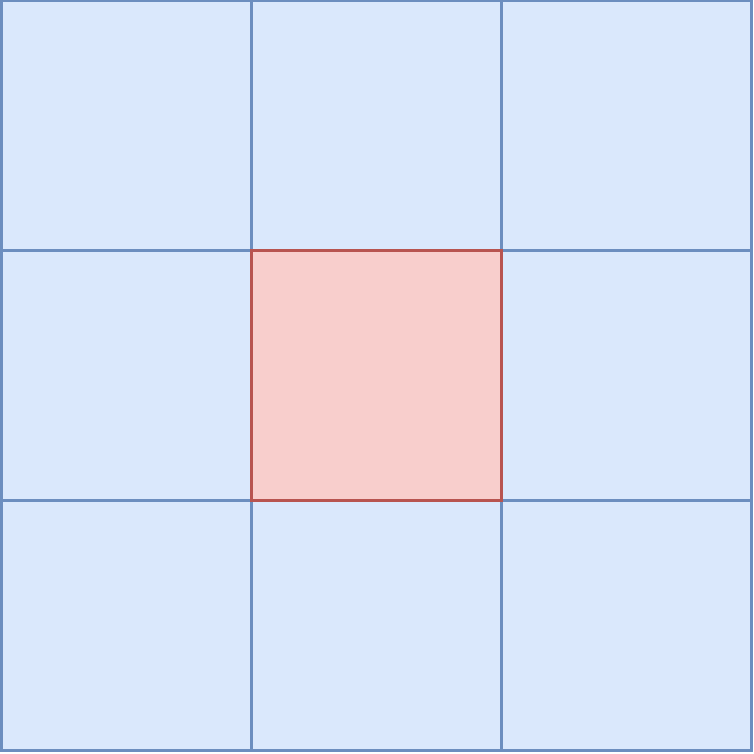
\includegraphics[width=0.3\columnwidth]{pics/moduleloop.pdf}}
\caption{A difficult scenario for adding a new module at red location}
\label{fig:loop}
\end{figure}

\begin{figure}[ht!]%[H]
\centering
{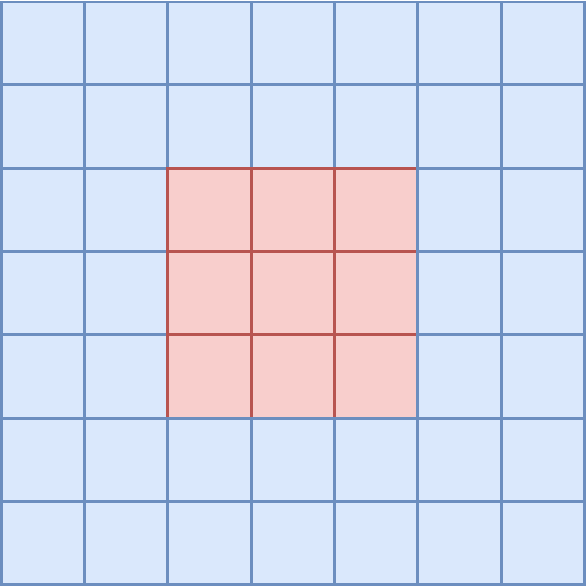
\includegraphics[width=0.3\columnwidth]{pics/moduleloop2.pdf}}
\caption{Modules in red cannot be distinguished}
\label{fig:loop2}
\end{figure}

\subsubsection{Search for starting region}
The starting region of the task is labeled with an AprilTag with an unique ID. Using the external camera, the task planner is able to find the positions and orientation of the starting point in the robot workspace. In this work, we choose the starting region to maximize the working area of the robot.

\subsubsection{Place the initial module to the starting region}
With the initial module and the starting region identified, the high-level planer then invoke the trajectory planner to control the robot to pick up the module and place it in the starting region.
When picking up a module, if the robot fails to grab the module, the task planner will receive the failure status from the trajectory planner and inform the user. The user can choose to retry or abort the task.

\subsection{Attach new modules}
\subsubsection{Select next module}\label{sec:nextmodule}


%The task planner in this work is based on the framework introduced in \cite{HKG2009}.
%A reactive robot task specification is expressed in LTL formulas.
%Then the specification is automatically transformed to a correct-by-construction discrete controller.
%At last, the controller is continuously implemented to generate desired robot behaviors.
%Different from \cite{HKG2009}, in this work we aim to synthesize controllers for multiple robots executing a manipulation task.
%Therefore, there are three main challenges in this work for task planning, as described in the following sections.
%
%\subsection{Specification Language for Multi-robot}
%In \cite{ChenDSB12,Diaz-MercadoJBE15}, the author introduces an approach for specifying robot tasks in formal language and generating controllers for a team of robots. 
%However, the type of robot tasks is limited to non-reactive, i.e. the environment is assume static and the robot behavior does not depend on the environment state.
%The framework in \cite{HKG2009} allows reactive robot task, such as "if the robot sense a soda can, bring the can to the kitchen".
%However, the task specification only issues commands for a single robot.
%In order to specify reactive tasks for a team of robots, we need to extend the specification language to able to express  multi-robot tasks.
%
%\subsection{Tasks Allocation}
%The framework employed in this work will generate a centralized controller for a team of robots.
%We will then distribute tasks to each robots in a synchronized process.
%One method is to handle task allocation in the high-level specification.
%Therefore, task distribution for each robot will be encoded in the synthesized controller.
%The drawback for this method is that, whenever a new task allocation is required,
%possibly due to failing to find a feasible trajectory, the entire discrete controller needs to be resynthesized.
%Another method for task allocation is to treat all robots as one virtual robot with multiple redundant action abilities.
%The specification will only describe tasks for this virtual robot,
%and the task allocation will be determined when executing the synthesized controller.
%The disadvantage of this method is that the algorithm will spend more time during execution for computing the task allocation plan.
%Both method will be implemented in this work.
%We will compare the performance of both methods and choose the better one.
%
%\subsection{Feedback from Trajectory Planner}
%Once task are allocated to each robot, the task planner will invoke the trajectory planner to move each robot arm to desired location without collision.
%In the situation where the trajectory planner fails to find a feasible path for an arm,
%it will provide feedback to the task planner about such failure.
%The task planner will then incorporate the information into the task specification and come up with a new discrete plan.
%If no plan can be created, the task planner will notify the user the possible cause of failure, e.g. the robot arm cannot reach the desire position. 